\subsection{ANOVA}

ANOVA is a statistical method used to compare the means of multiple groups to see if there are any significant differences among them. It is especially helpful when you have one or more categorical variables (like season or district) and a continuous outcome (like temperature).

\subsection*{Key Concepts}

\begin{itemize}
    \item \textbf{Null Hypothesis (H\textsubscript{0}):} All group means are the same — no real difference between groups.
    
    \item \textbf{Alternative Hypothesis (H\textsubscript{1}):} At least one group mean is different from the others.
    
    \item \textbf{F-Statistic:} This number compares how much the groups differ compared to the variability inside each group. A larger F-value means more likely there is a real difference.
    
    \item \textbf{p-value:} If this value is less than 0.05, we reject the null hypothesis, meaning there is a significant difference between some groups.
    
    \item \textbf{Effect Size ($\eta^2$ or Partial $\eta^2$):} This tells us how much of the change in the dependent variable is explained by the groups — basically, how strong the effect is.

\end{itemize}

\subsection*{How to Perform ANOVA}

\begin{enumerate}
    \item Click on \textbf{ANOVA} from the top menu.
    \item Under \textbf{Classical}, select \textbf{ANOVA}.
    \item Drag your continuous variable (e.g., Temp 2m) into the \textbf{Dependent Variable} box.
    \item Drag your categorical variable(s) (e.g., Season, District) into the \textbf{Fixed Factors} box.
    \item To study interaction effects (how factors work together), select more than one fixed factor (e.g., District × Season).
    \item Choose \textbf{Homogeneity Tests} (like Levene’s test) to check if the groups have similar variances.
    \item Click \textbf{Effect Size ($\eta^2$)} to see the strength of the relationship.
\end{enumerate}

% Figure here-----------------------------
\begin{figure}[h]
\centering
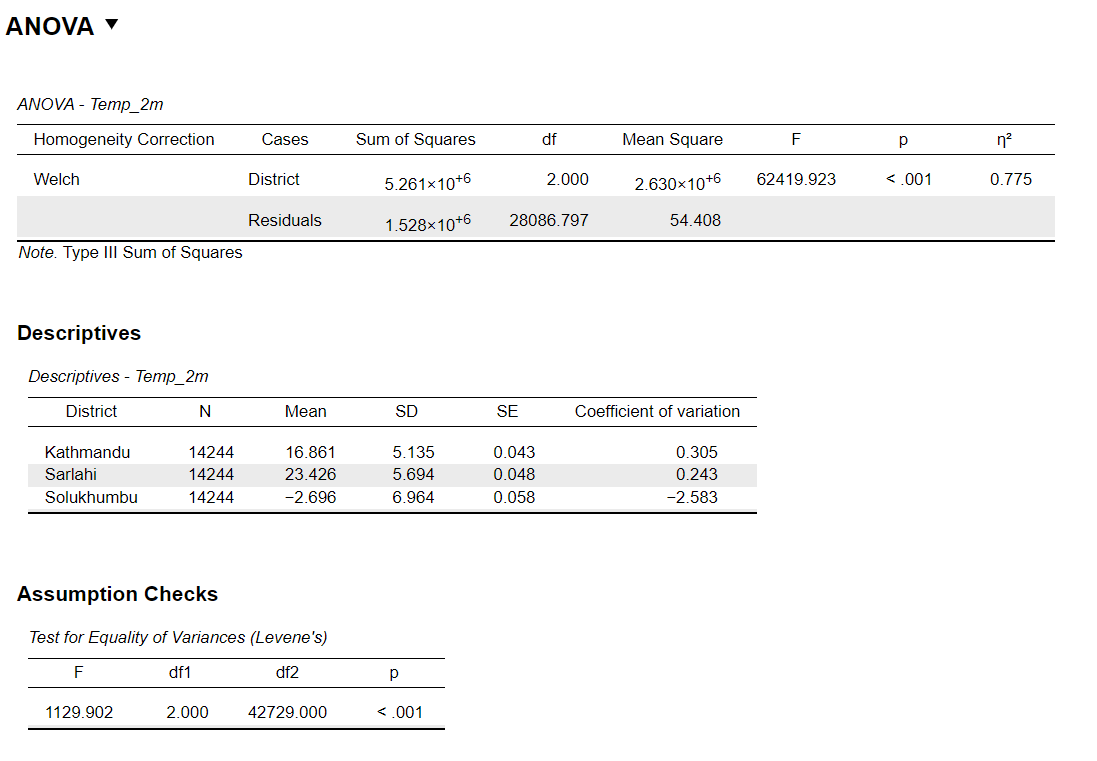
\includegraphics[width=0.7\textwidth]{figures/ANOVA.png}
\caption{ANOVA}
\end{figure}

\textbf{InterPretation:}
\begin{itemize}
    \item \textbf{Main Effect – District}
    \begin{itemize}
        \item Temperature varies significantly across the three districts.
        \item $F = 62{,}419.923$, $p < .001$ — the difference is statistically significant.
        \item $\eta^2 = 0.775$ — very large effect size, meaning 77.5\% of the temperature variation is explained by the district.
    \end{itemize}
    
    \item \textbf{Unexplained (Residual) Variance}
    \begin{itemize}
        \item Some variation in temperature remains unexplained.
        \item Residual sum of squares = $1{,}528{,}000$ (approx).
    \end{itemize}
    
    \item \textbf{Average Temperatures in Each District}
    \begin{itemize}
        \item \textbf{Sarlahi}: Hottest (around $23.4^\circ$C)
        \item \textbf{Kathmandu}: Moderate (around $16.9^\circ$C)
        \item \textbf{Solukhumbu}: Coldest (around $-2.7^\circ$C )(likely due to high elevation)
    \end{itemize}
    
    \item \textbf{Assumption Check(Levene’s Test)}
    \begin{itemize}
        \item $F = 1129.902$, $p < .001$ — indicates variances are not equal across districts.
        \item Because of this, Welch’s ANOVA (which doesn’t require equal variances) was used for better accuracy.
    \end{itemize}
\end{itemize}
